%%%%%%%%%%%%%%%%%%%%%%%%%%%%%%%%%%%%%%%%%
% a0poster Portrait Poster
% LaTeX Template
% Version 1.0 (22/06/13)
%
% The a0poster class was created by:
% Gerlinde Kettl and Matthias Weiser (tex@kettl.de)
% 
% This template has been downloaded from:
% http://www.LaTeXTemplates.com
%
% License:
% CC BY-NC-SA 3.0 (http://creativecommons.org/licenses/by-nc-sa/3.0/)
%
%%%%%%%%%%%%%%%%%%%%%%%%%%%%%%%%%%%%%%%%%

%----------------------------------------------------------------------------------------
%	PACKAGES AND OTHER DOCUMENT CONFIGURATIONS
%----------------------------------------------------------------------------------------

\documentclass[a0,portrait]{a0poster}
\usepackage[font=small,labelfont=bf]{caption}
\usepackage{multicol} % This is so we can have multiple columns of text side-by-side
\columnsep=50pt % This is the amount of white space between the columns in the poster
\columnseprule=3pt % This is the thickness of the black line between the columns in the poster
\usepackage{easySymbols}
\usepackage{wrapfig}
\usepackage[svgnames]{xcolor} % Specify colors by their 'svgnames', for a full list of all colors available see here: http://www.latextemplates.com/svgnames-colors
\usepackage[utf8]{inputenc}
\usepackage{times} % Use the times font
%\usepackage{palatino} % Uncomment to use the Palatino font

\usepackage{graphicx} % Required for including images
\graphicspath{{figures/}} % Location of the graphics files
\usepackage{booktabs} % Top and bottom rules for table
\usepackage[font=small,labelfont=bf]{caption} % Required for specifying captions to tables and figures
\usepackage{amsfonts, amsmath, amsthm, amssymb} % For math fonts, symbols and environments
\usepackage{wrapfig} % Allows wrapping text around tables and figures

\begin{document}

%----------------------------------------------------------------------------------------
%	POSTER HEADER 
%----------------------------------------------------------------------------------------

% The header is divided into two boxes:
% The first is 75% wide and houses the title, subtitle, names, university/organization and contact information
% The second is 25% wide and houses a logo for your university/organization or a photo of you
% The widths of these boxes can be easily edited to accommodate your content as you see fit

\begin{minipage}[b]{\linewidth}
\veryHuge \color{NavyBlue} \textbf{Perturbation-based gene regulatory network inference to unravel oncogenic mechanisms} \color{Black}\\ % Title
% \Huge\textit{to uncover Oncogenic Mechanisms}\\[2cm] % Subtitle
% \huge \textbf{John Smith \& James Smith}\\[0.5cm] % Author(s)
% \huge University and Department Name\\[0.4cm] % University/organization
% \Large \texttt{john@LaTeXTemplates.com} --- 1 (000) 111 1111\\
\huge \textbf{ Daniel Morgan$^1$, Matt Studham$^1$, Andreas Tj\"{a}rnberg$^2$, Bo Lundgren, Fredrik Swartling, Torbj\"{o}rn  Nordling$^3$, Erik Sonnhammer$^1$ } \\[0.1cm]
\large $^1$\it {DBB, Stockholm University \& SciLifeLab} $^2$\it{Department of Bioinformatics, Link\"{o}ping University} $^3$\it {Mechanical Engineering, National Cheng Kung University} $^4$\it \\[0.4cm]
\Large \texttt{Daniel.Morgan@SciLifeLab.se}
\end{minipage}
%
% \begin{minipage}[b]{0.25\linewidth}
% \includegraphics[width=10cm]{logo.png}\\
% \end{minipage}

\vspace{1cm} % A bit of extra whitespace between the header and poster content

%----------------------------------------------------------------------------------------

\begin{multicols}{2} % This is how many columns your poster will be broken into, a portrait poster is generally split into 2 columns

%----------------------------------------------------------------------------------------
%	ABSTRACT
%----------------------------------------------------------------------------------------

\color{Navy} % Navy color for the abstract

% \section*{abstract}

\noindent\textbf{Motivation:} Cancer is known to stem from multiple, independent mutations, the effects of which aggregate to drive the cell into a cancerous state. To understand the complex interplay between affected genes, their gene regulatory network (GRN) needs to be uncovered, revealing detailed insights of regulatorymechanisms. We therefore decided to infer a reliable GRN from perturbation responses of 40 genes known or suspected to have a role in human cancers yet whose regulatory interactions are poorly known. \\
\textbf{Results:} siRNA knock-down experiments of each gene were done in a human squamous carcinoma cell line, after which the transcriptomic response was measured. From these data GRNs were inferred using several methods, and the false discovery rate was controlled by the NestBoot framework. The best GRN's topology was validated by measuring its ability to predict an independent dataset of the same genes but subjected to double perturbations. It agrees with many known links in addition to predicting a large number of novel interactions, a subset of which were experimentally validated. The inferred GRN captures regulatory interactions central to cancer-relevant processes and thus provides mechanistic insights that are useful for future cancer research. 
\color{Black}

%----------------------------------------------------------------------------------------
%	INTRODUCTION
%----------------------------------------------------------------------------------------

% \color{SaddleBrown} % SaddleBrown color for the introduction

\section*{Background}
Cancer is, in part, a progressive, systemic flux of cellular functions driven by the interaction of multiple gene products \cite{subramanian2017next}\cite{barabasi2011network} from a more general state of non-cancer. Cancer subtype-specific gene regulatory networks (GRN) encode intracellular dynamics \cite{tarca2006analysis}, thus understanding them can offer insight into the functional changes driving disease development. %Several approaches exist for this reverse engineering, ranging from an outdated assembly of one-to-one relationships to correlating patterns throughout expression assays and more. %As with all analysis, the underlying experimental techniques, setup and data quality are non-trivial elements for the quality of inferred models. 
Generally, such inference methodologies are designed to exploit certain aspects of the experimental setup, such as pooling among replicates to amplify signal, or make use of prior knowledge \cite{haury2012tigress} \cite{mordelet2008sirene}. However methods often fall short of guarding against limitations of the experimentation, such as poor estimations of biological variation which can lead to overfitting and potentially contributes to the inconsistencies seen among benchmarks \cite{guo2016gene}. Methods using systematic perturbation have shown greater accuracy among inference techniques since more information is available to determine regulatory causal mechanism in the system \cite{minnier2011perturbation}. %In this study, data is collected from such gene knockdown in order to measure the global influence of each individual gene in a more wild type system, rather than through irreversible and complete knockout. 
Assuming a linear dynamical system (LDS) \cite{gardner2003inferring} model, once the system has reached a steady-state equilibrium the network can be inferred  by , solving a set of  linear ordinary differential equations (ODEs). 

%----------------------------------------------------------------------------------------
%	OBJECTIVES
%----------------------------------------------------------------------------------------

% \color{DarkSlateGray} % DarkSlateGray color for the rest of the content

% \section*{Main Objectives}

% \begin{enumerate}
% \item Removed batch and other sources of unwanted noise from L1000 dataset.
% \item Infer networks per cell line \& as a {\it generic} aggregate.
% \item Compare subtype networks link-wise.
% \item Investigate liver cancer subnetwork.
% \end{enumerate}

%----------------------------------------------------------------------------------------
%	MATERIALS AND METHODS
%----------------------------------------------------------------------------------------

\section*{Methods}

\begin{equation*}\label{eq:Linearmap}
\text{\textbf{Linear Model:}} \qquad\qquad\qquad\qquad \mY = -\mA^{-1}(\mP+\mF)+ \mE
\end{equation*}

  \begin{equation*}
 \text{\textbf{Inference Method 1: LSCO}} \qquad\qquad\qquad \hat{A}_{LS}={{X^TX}^{-1} X^Ty}
 \label{eq:LSCO}
 \end{equation*}
 
  \begin{equation*}
 \text{\textbf{Inference Method 2: LASSO}} \qquad \min_{w \in \mathbb{R}p}
 \frac{1}{2m} \norm{\mA_i\mY^T+\mP^T_i}^2_F + \zeta \norm{\mA}_1
 \label{eq:LASSO}
 \end{equation*}
 
 \begin{equation*}
  \text{\textbf{Inference Method 3: TLSCO}} \qquad\qquad\qquad
  \begin{aligned}
%     \svd
    \lbrack X Y\rbrack &= U S V , \\
    \hat{A}_{TLS} &= -\frac{VXY}{VYY}
 \label{eq:TLSCO}
  \end{aligned}
 \end{equation*}

\begin{center}
\includegraphics[width=.65\linewidth]{MYC_alg.png}
\end{center}

% \section*{Methods B}
\begin{center}
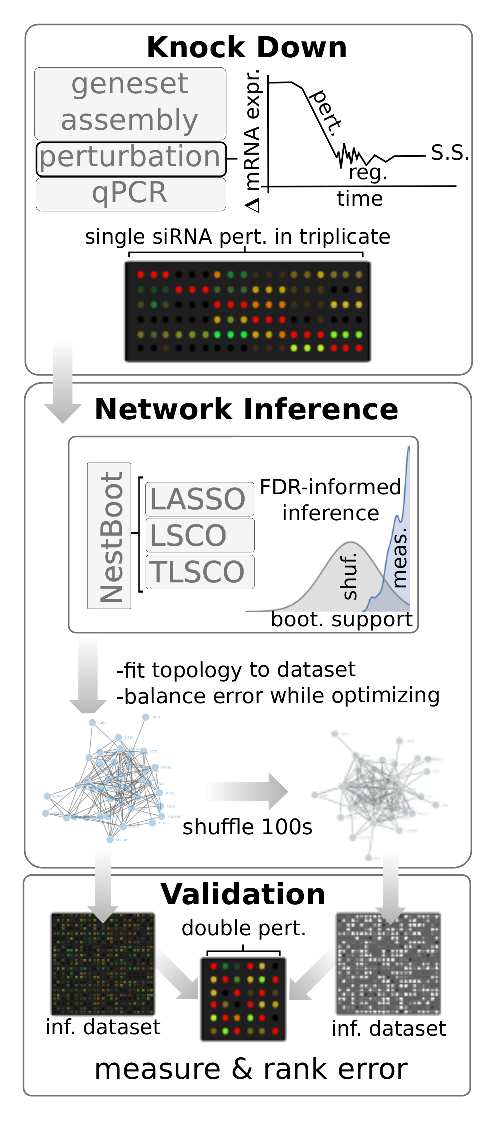
\includegraphics[width=.6\linewidth]{MYC_analysis_C.eps}
\end{center}

%----------------------------------------------------------------------------------------
%	RESULTS 
%----------------------------------------------------------------------------------------

\section*{Results}


\begin{center}
% \hspace{.25cm}\vspace{.1cm}
\includegraphics[width=.59\linewidth]{MYC_perf.png}
\includegraphics[width=.39\linewidth]{LASSO_1145.png}
\end{center}
% \vspace{-.3cm}
%----------------------------------------------------------------------------------------
%	CONCLUSIONS
%----------------------------------------------------------------------------------------





%----------------------------------------------------------------------------------------
%	FORTHCOMING RESEARCH
%----------------------------------------------------------------------------------------

% \section*{Forthcoming Research}

% Incorporation of small molecule perturbation may offer novel drug-target predictions for each cancer subtype.

 %----------------------------------------------------------------------------------------
%	REFERENCES
%----------------------------------------------------------------------------------------



%----------------------------------------------------------------------------------------
%	ACKNOWLEDGEMENTS
%----------------------------------------------------------------------------------------


%----------------------------------------------------------------------------------------

\end{multicols}
\color{SaddleBrown} % SaddleBrown color for the conclusions to make them stand out

\section*{Conclusions}

\begin{itemize}
\item A common set of genes was perturbed and measured independently in human squamous carcinoma cell line. 
\item The training dataset contains genes perturbed and measured three times as experimental replicates, while the validation dataset contains the same genes perturbed in pairs without replicate. 
\item Taking into account various data properties, the training dataset was used to infer a network of the underlying mechanisms of control. 
\item This network was able to reproduce its training data in a leave out manner, and whatsmore, it is robust enough to reproduce a separate validation dataset to a degree of accuracy higher than expected by chance. 
\item In this way, many known links were recovered during the inference, as well as novel links proposed, two of which were verified experimentally.
\end{itemize}

\color{DarkSlateGray}
\bibliographystyle{plain} 
\small \bibliography{references.bib} 
\end{document}